\documentclass[../Thesis.tex]{subfiles}
\graphicspath{{\subfix{../figures/}}}
% \epstopdfsetup{outdir={../figures/}}
\begin{document}
% effects of scaling g_obs
% "bevis" for antagelse ikke holder for e.g. normalfordeling, men numerisk hvorfor det går godt??
% Hvad hvis man sætter entropi i diagonalen i stedet for 0? eller 1 hvis correlation. Undersøg numerisk.
% for at øge computer stabilitet kan G_obs skaleres til den har spektral radius mindre end 1. Spektrum/egenværdier numerisk mindre end 1
% $\rho\left(G_{obs}\right) < 1$ ??

% UNDERSØG: bruger original artikel at spektral radius af G_obs skal være mindre end 1? Det skal den ikke
% Det følger af proposition 5.3 / corrolary 5.2.1 at for en 1D manifold, under grænseværdien, at MI bare kan regnes som entropi for 1 af variablene (hvis det er 1-to-1??)

% Det er en vigtig del af correlation og MI at de virker for mixed variables. MI virker fordi continuert er grænsen for en diskretisering af en kontinuert variabel, så giver mening definitionsmæssigt at sammenligne kontinuert og diskret MI.


\chapter{Method}

\section{Causal discovery}
In this section, we shall discuss the method for network deconvolution, originally proposed by \cite{Network-deconvolution-as-a-general-method-to-distinguish-direct-dependencies-in-networks}. The underlying problem is inferring direct effects and dependencies. From this, using prior information on the production setup, we shall be able to infer causal dependencies by directing the resulting edges from the network deconvolution (ND) algorithm. Particularly, the framework and general algorithm proposed Feizi et al. stems from a graph-theoretic approach to the problem of inferring direct dependencies. Namely, suppose that observations are made of some properties of in this case a chemical process. We shall represent these properties as vertices (nodes) $V$ and dependencies between properties as edges. Initially, when observing the vertices, we observe both direct and indirect effects. Particularly, a vertex $v_1$ might influence some other vertex $v_3$ through another vertex $v_2$ if $v_2$ depends on $v_1$ and $v_3$ of $v_2$. In this case, we will observe that $v_1$ influences $v_3$, but actually it is $v_2$ that has a direct influence on $v_3$. In graph-theoretical terms, we thus observe the transitive closure of the information that flows between vertices but want to infer the underlying network structure.

An important note on the algorithm to come is that we only use vertices that we have observed. Namely, the underlying structure might be as in \autoref{subfig:hidden nodes example unobserved} with an unobserved node/variable (named $U$ in this case). However, without any more assumptions or modelling choices we would (ideally) infer the network structure depicted in \autoref{subfig:hidden nodes example resulting graph}.
\begin{figure}[h]
    \centering
    \begin{subfigure}[t]{0.49\textwidth}
        \centering
        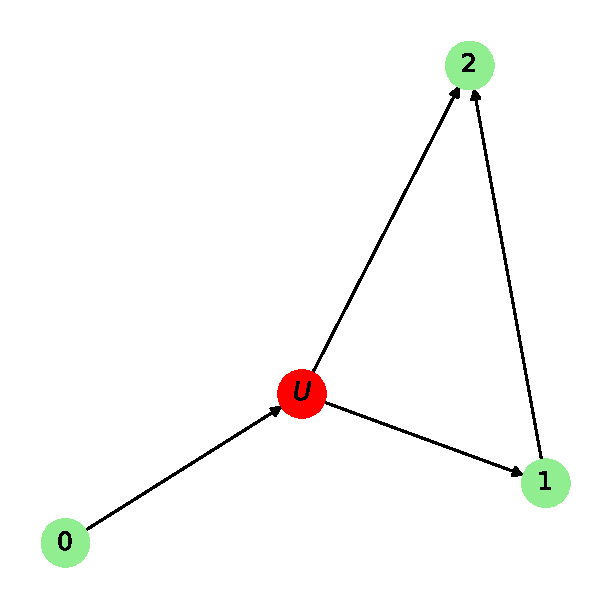
\includegraphics[width=\linewidth]{figures/ND examples/Hidden nodes/graph example w hidden.pdf}
        \caption{}
        \label{subfig:hidden nodes example unobserved}
    \end{subfigure}
    %
    \begin{subfigure}[t]{0.49\textwidth}
        \centering
        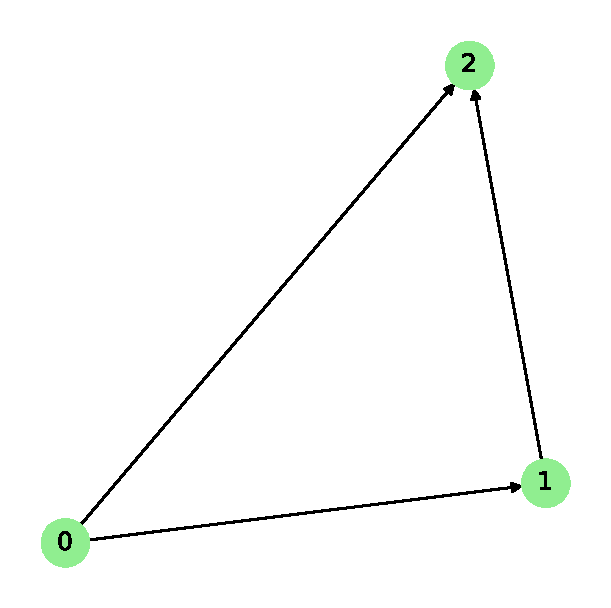
\includegraphics[width=\linewidth]{figures/ND examples/Hidden nodes/graph example wo hidden.pdf}
        \caption{}
        \label{subfig:hidden nodes example resulting graph}
    \end{subfigure}
    \caption{(a) An example of a causal structure depicted as a graph. When observing the network, only nodes $0$, $1$ and $2$ are observed/recorded. (b) The resulting inferred graph from observational data. Although this is not a complete picture of the true underlying dynamics of the system, if only the observed variables are of interest, this will be an equally proper representation of the system. Furthermore, in practice this means no further assumptions are made which can and can not be of desire. Namely, if prior information is accessible one might introduce new nodes in the inferred network.}
    \label{fig:hidden nodes example}
\end{figure}
With these initial comments, we proceed with the general setup and assumptions for network deconvolution based on observations.

\subsection{Setup and assumptions}
Suppose a set of $N$ random variables $(X_i)$ is given. The method presented in this section aims to discover direct relationships between pairs $X_i$ and $X_j$ for $i\neq j$. These relationships will be presented by an undirected graph as in the previous section. In particular, we shall let each random variable $X_i$ be represented by a vertex in a graph. We will later discuss a way of directing edges such that a causal network may be discovered i.e. a directed acyclic graph that may be used for inference.

The method proposed by \cite{Network-deconvolution-as-a-general-method-to-distinguish-direct-dependencies-in-networks} then works as follows. Given an observed matrix $G_{obs} \in \mathbb{R}^{N \times N}$ of similarities between each pair of variables, we shall deduce a matrix $G_{dir} \in \mathbb{R}^{N \times N}$ of direct similarities between each pair of random variables $X_i$ and $X_j$. The measure of similarity, can in practice be any desired measure such a correlation, mutual information which we will focus on in this thesis. See \autoref{seq:Information measures and computation} for a further discussion on these two measures. Note that the algorithm presented will in theory work for non-symmetric measures as well such as \textit{Interaction information}, \textit{Directed information} and \textit{Normalized information}.

The (direct) network is then presented by the discovered $G_{dir}$ containing only the direct effects i.e. interaction between pairs of variables which can be viewed as weights on the edges of the complete graph with nodes representing the random variables. As we shall see in section \autoref{subseq:Robustness to noise}, the algorithm is somewhat robust to noise in the sense that we can ensure accuracy depending on the level of noise observed present in $G_{obs}$ and on the norm chosen (from a certain, although rather general, set of norms). This hints to that a threshold on the inferred weights on the edges of the network might be a good idea which is further solidified by the facts that often only the most influential variables are of importance when trying to control the process.

The first assumption is that the observed matrix of co-dependence $G_{obs}$ may be expressed as
\begin{equation}
    G_{obs} = G_{dir} + G_{indir}
\end{equation}
Namely, that the direct and indirect effects can be added together to get the total and thus observed interdependence between each pair of variables. Often, this is not the case as we shall see later on. However, the error made from this assumption and the ones to be presented seem to be small enough that the discovered network accurately resemble the true underlying network.

The second and final assumption is that the indirect effects $G_{indir}$ can be computed in terms of $G_{dir}$. Namely, that
\begin{equation}
    G_{indir} = G_{dir}^2 + G_{dir}^3 + \dots
\end{equation}
i.e. that the observed \textit{information} exchanged on an edge $e_{ij}$ between nodes $X_i$ and $X_j$ is the sum second, third etc. order effects, each given by the information on the $n$-path (where $n$ is the order of the (diminishing) indirect effect) again assumed to a sum of products. In other terms, the second order indirect effect between $X_i$ and $X_j$ (given as the $(i,j)$ element of $G_{dir}^2$) is the sum of products on edges $e_{ik}$ and $e_{kj}$ for all $k$
$$\left[G_{dir}^2\right]_{ij} = \sum_{k=1}^N e_{ik}\,e_{kj}$$
where $e_{ij}$ is the $(i,j)$ element of $G_{dir}$. Immediately, we observe that $e_{ii}$ is of interest in terms of its physical meaning. The co-dependence between a random variable and itself might be somewhat ambiguous or even undefined depending on the measure. Thus, the meaning of (non-existing) edges $e_{ii}$ will be of interest later on when using the method on controlled cases to see if any sense can be made of these.

Thus, from the above assumptions, it follows that we can express $G_{obs}$ as
\begin{equation}
    G_{obs} = G_{dir} + G_{dir}^2 + G_{dir}^3 + \dots
\end{equation}
Hence, for $G_{dir}$ to exist, it must have spectral radius at most $1$ as otherwise, the above sum diverges and thus $G_{obs}$ will not exist. I.e. $\rho\left(G_{dir}\right) < 1$. Thus, assuming convergence we can rewrite the infinite series as
\begin{equation}\label{eq:Gobs from Gdir}
    G_{obs} = G_{dir} \left(I - G_{dir}\right)^{-1}
\end{equation}
It immediately follows that $G_{dir}$ is given by (can be proved by directly inserting the above expression for $G_{obs}$)
\begin{equation}
    G_{dir} = G_{obs} \left(I + G_{obs}\right)^{-1}
\end{equation}
Furthermore, if the measure of dependence between pairs of variables is symmetric, then so is $G_{obs}$ and hence diagonalizable by some orthogonal matrix $U$ such that $G_{obs} = U \Lambda_{obs} U^T$ (with the columns of $U$ being eigenvectors of $G_{obs}$). It follows that $G_{dir}$ can be expressed in a simple (and later computationally efficient) way
$$G_{dir} = U \Lambda_{dir} U^T$$
where $\Lambda_{dir} = \Lambda_{obs} \left(I + \Lambda_{obs}\right)^{-1}$.

We note that from the above one needs $\left( I + G_{obs}\right)^{-1}$ to be well-defined which is equivalent to $-1 \not\in \sigma_{G_{obs}}$ i.e. $-1$ is not an eigenvalue of $G_{obs}$. To see that this is indeed the case whenever $\rho\left(G_{dir}\right) < 1$, and that $I + G_{obs}$ is thus invertible we use \autoref{eq:Gobs from Gdir} and simplify
\begin{align*}
    I + G_{obs} & = I + G_{dir} \left(I-G_{dir}\right)^{-1}                                                \\
                & = \left(I-G_{dir}\right)\left(I-G_{dir}\right)^{-1} + G_{dir}\left(I-G_{dir}\right)^{-1} \\
                & = \left(I-G_{dir}\right)^{-1}
\end{align*}
which is clearly invertible. Furthermore, we note that under the assumption $\rho\left(G_{dir}\right) < 1$ we can not place any bound on the spectral radius of $G_{obs}$. Namely, if $v$ is a unit eigenvector of $G_{dir}$ with eigenvalue $\lambda$ such that $|\lambda|<1$, then $v$ is also an eigenvector of $G_{obs}$ as
$$G_{obs} v = \sum_{k=1}^\infty G_{dir}^k v = \sum_{k=1}^\infty \lambda v = \frac{\lambda}{1-\lambda} v$$
i.e. $\left(\frac{\lambda}{1-\lambda},v\right)$ is an eigenpair of $G_{obs}$ and since $\frac{\lambda}{1-\lambda} \in (-1/2, \infty)$ for $\lambda\in (-1,1)$ we can in general not bound the spectral radius of $G_{obs}$, although we should never observe an eigenvalue equal to or below $-1/2$ (which again proves that $-1$ is not an eigenvalue of $G_{obs}$).

Now, before discussing the implementation and analyzing the algorithm both analytically and through examples, we will take a closer look at the similarity measures that are to be used with this method and that in the end will make up the matrix $G_{obs}$. Namely, \textit{mutual information} and \textit{correlation}.


\section{Information measures and computation}\label{seq:Information measures and computation}
In this section we discuss two measures that can be used to construct the matrices of codependency from the previous section. Namely, we shall touch on correlation and discuss what one might choose to call Copula-based entropy. However, before discussing Copula entropy (CE) we first need to define what a copula is.

\subsection{Copula}
Given a set of $N$ random variables $X_1,\dots, X_N$, a copula is loosely speaking a distribution function with support $[0,1]^N$ incorporating the dependence structure between the random variables. Given a joint distribution function $F$ and (invertible) marginals $F_1,\dots,F_N$ we define a copula $C$ as
$$F(x_1,\dots,x_N) = \mathbb{P}\left(X_1\leq x_1,\dots, X_N\leq x_N\right) = C\left(F_1\left(x_1\right),\dots,F_N\left(x_N\right)\right)$$
Letting $u_i = F_i\left(x_i\right) \in [0,1]$ it is clear that $C$ is a distribution function as described above \cite{Copula-handbook}. Furthermore, it follows that the marginals of $C$ are uniform. We thus define a copula in probabilistic terms as
\begin{definition}[Copula]\label{def:copula}
    A function $C:[0,1]^d \to [0,1]$ is called a copula if it has uniform marginals and is a distribution function for a $d$-dimensional random vector $\mathbf{X}$.
\end{definition}
An important and fundamental theorem of copulas for especially continuous random variables where the marginals are also continuous functions is stated by Sklar:
\begin{theorem}[Sklar's theorem] \label{thm: Sklar}
    For a random vector $\boldsymbol X$ with CDF $F$ and univariate marginal CDFs $F_1, \dots, F_d$. There exists a copula $C$ such that
    \begin{equation}\label{eq:sklar}
        F(x_1,\dots,x_d) = C(F_1(x_1), \dots, F_d(x_d))
    \end{equation}
    If $X$ is continuous, $C$ is unique; otherwise $C$ is uniquely determined on the Cartesian product of the ranges of distribution functions $F_i$, $\prod \text{Ran}\left(F_i\right)$.
\end{theorem}
Note that the last statement for non-continuous random variables can be made unique by instead using subcopulas, a generalization of copulas with domain $I$ only a subdomain of the unit hypercube $\mathbb{I}^d = [0,1]^d$ containing all faces of the unit hyper cube. However, there are infinitely many ways of extending such a subcopula to a copula $C$\cite{Copula-modeling-for-discrete-random-vectors}. In our case, this means that for discrete and/or mixed variables, we will later have to work around this non-uniqueness when calculating mutual information. The example made by Geenens\cite{Copula-modeling-for-discrete-random-vectors} is a bivariate random vector of independent variables $X \sim \text{Bern}\left(\pi_X\right)$ and $Y\sim \text{Bern}\left(\pi_Y\right)$. The support of $F_X$ and $F_Y$ is then $\{0, 1-\pi_X\}$ and $\{0, 1-\pi_Y\}$ respectively. Due to the restriction on the boundary of the unit square, the only unique point of a copula $C$ is then $(1-\pi_X, 1-\pi_Y)$, and by independence we must have
$$C\left(1-\pi_X, 1-\pi_Y\right) = (1-\pi_X)( 1-\pi_Y)$$
Geenens then proceed to define an uncountable set of copulas that fulfill the above criterion which further illustrates that the basic concepts of copulas are not well suited for discrete random vectors. Note that in the article it is however argued how one can extend the concept to a more general concept that works for mixed variables.

From \autoref{eq:sklar} we see that a copula is thus simply just a function that \textit{couples} the marginals of a random vector to the joint distribution. The following corollary follows immediately
\begin{corollary}[Coordinate transformation] \label{coro: Coordinate transformation}
    Under the assumptions of \autoref{thm: Sklar}, given any set $(T_1, \dots, T_d)$ of strictly increasing functions, if $C$ is a copula of $(X_1,\dots, X_d)$ then it is also a copula of $(T_1(X_1), \dots, T_d(X_d))$.
\end{corollary}
\begin{proof}
    Suppose $(X_1 , \dots , X_d)$ permits a copula $C$ and let $T_i$ be given as stated. Consider coordinate wise the result of the transformation $Y_i = T_i(X_i)$ and consider the CDF $F_{Y_i}(y_i)$
    $$F_{Y_i}(y_i) = \mathbb{P}\left(Y_i \leq y_i\right) = \mathbb{P}\left(T_i^{-1}(Y_i) \leq T_i^{-1}(y_i)\right) = \mathbb{P}\left(X_i \leq x_i\right) = F_{X_i}(x_i)$$
    Thus
    \begin{align*}
        F_{\boldsymbol X} (x_1,\dots , x_d) & = C\left( F_{X_1}(x_1), \dots, F_{X_d}(x_d)\right) \\
                                            & = C\left( F_{Y_1}(y_1), \dots, F_{Y_d}(y_d)\right) \\
                                            & = F_{\boldsymbol Y}(y_1, \dots, y_d)
    \end{align*}
    where Sklar's theorem have been used for the final equality.
\end{proof}
The above corollary is actually equivalent with a seemingly stronger statement and follows easily
\begin{proposition}
    Since $T_i$ is strictly increasing, the inverse $T_i^{-1}$ exists and is also strictly increasing. Thus, the above implication is bidirectional and hence for strictly increasing functions $T_i$, $C$ is a copula of $\left(X_1,\dots,X_d\right)$ if and only if it is a copula of $\left(T_1(X_1),\dots, T_d(X_d)\right)$.
\end{proposition}


\textcolor{red}{casuality svarer til at lave nedre/øvre trekant. Er der forskel i at gør edet før og efter for en symmetrisk matrix?}



\subsection{Mutual information and Copula entropy}
In this section we introduce Copula entropy as done in \cite{Nonparametric-copula-entropy-and-network-deconvolution-method-for-causal-discovery-in-complex-manufacturing-systems} and see how it actually is equal to the well known mutual information. The name comes from the general definition of (differential) entropy as we shall see shortly. However, first we define mutual information between a set of random variables
\begin{definition}[Mutual information]\label{def:mutual information}
    For a discrete random vector $\boldsymbol{X} = \{X_i\}$, we define the mutual information as
    $$I(\boldsymbol{X}) = \sum_{\boldsymbol{x} \in \mathcal{X}} f(\boldsymbol{x}) \, \log_b\left(\frac{f(\boldsymbol{x})}{\prod_{i} f_i\left(x_i\right)}\right)$$
    where $\mathcal{X}$ is the domain of the random vector $\boldsymbol{X}$ and $f$ is the joint probability mass function with marginals $f_i$. Similarly, for continuous random vectors with $f$ the joint probability density function we define
    $$I(\boldsymbol{X}) = \int_{\boldsymbol{x} \in \mathcal{X}} f(\boldsymbol{x}) \, \log_b\left(\frac{f(\boldsymbol{x})}{\prod_{i} f_i\left(x_i\right)}\right)\, d\boldsymbol{x}$$
    where the base of the logarithm $b$ is often chosen to be $2$, $e$ or $10$ although the choice is unimportant as all logarithms are equivalent up to a scaling factor.
\end{definition}
\textcolor{red}{As we shall see later, the continuous version is the limit of the discrete version}

We immediately proceed with defining both entropy and differential entropy
\begin{definition}[Entropy]\label{def:entropy}
    The (joint) entropy of a discrete random vector $\boldsymbol{X}$ is defined as
    $$H\left(\boldsymbol{X}\right) = - \sum_{\boldsymbol{x}\in \mathcal{X}} f(\boldsymbol{x}) \, \log_b f(\boldsymbol{x})$$
\end{definition}

\begin{definition}[Differential entropy]\label{def:differential entropy}
    The (joint) differential entropy defined for a continuous random vector $\boldsymbol{X}$ is defined as
    $$h(\boldsymbol{X}) = - \int_{\boldsymbol{x} \in \mathcal{X}} f\left(\boldsymbol{x}\right) \, \log_b f\left(\boldsymbol{x}\right) \, d\boldsymbol{x}$$
\end{definition}

\textcolor{red}{We shall see shortly that these are not the limit of each other (discrete to continuous) but when using MI it does not matter and even makes implemtaiton simpler}


\begin{align*}
    I\left(\boldsymbol{X}\right) & = \int_{\boldsymbol{x} \in \mathcal{X}} f\left(\boldsymbol{x}\right) \, \log_b f\left(\boldsymbol{x}\right) \, d\boldsymbol{x} - \sum_{i = 1}^{d} \int_{\boldsymbol{x} \in \mathcal{X}} f\left(\boldsymbol{x}\right) \, \log_b f_i\left(x_i\right) \, d\boldsymbol{x}\\
    & = \int_{\boldsymbol{x} \in \mathcal{X}} f\left(\boldsymbol{x}\right) \, \log_b f\left(\boldsymbol{x}\right) \, d\boldsymbol{x} - \sum_{i = 1}^{d} \int_{x_i \in \mathcal{X}_i} f_i\left(\boldsymbol{x}\right) \, \log_b f_i\left(x_i\right) \, d x_i\\
    &= \sum_{i=1}^{d} h\left(X_i\right) - h\left(\boldsymbol{X}\right)
\end{align*}
and similarly for the discrete variant.


where the base $b$, initially, can be chosen at will as all logarithms are equal up to a scalar multiple of each other.




\textcolor{red}{forskellige baser og egentlig ikke et rigtigt valg. Dog er det forskellig skallering af G obs som vi senere viser har en effekt på højere ordens led. Kommenter på/henvis til dette i senere afsnit.}


However, to make the calculations more robust and efficient we will use a closely related measure of dependence, namely CE which is defined as follows
$$ CE\left(X_1,\dots, X_n\right) = -\int \dots \int_{[0,1]^n} c\left(u_1,\dots, u_n\right) \log_{b}c\left(u_1,\dots, u_n\right) \, d u_1 \dots d u_n$$
where $c(\cdot)$ is the uniquely defined copula density of the joint distribution $f_{\mathbf{X}}(\cdot)$. We show that the above is indeed equal to the negative mutual information. First, we realize that from definition,
\begin{align*}
    c(u_1,\dots , u_n) & = \partial_{\mathbf{u}} C(u_1,\dots,u_n)                                                        \\
                       & = \partial_{\mathbf{u}} F\left(F_1^{-1}\left(u_1\right), \dots, F_n^{-1}\left(u_n\right)\right) \\
                       & = f\left(x_1,\dots, x_n\right) \frac{1}{f_1(x_1)\dots f_n(x_n)}
\end{align*}
Thus
\begin{align*}
    -CE & = \int\dots \int_{[0,1]^n} c\left(u_1,\dots, u_n\right) \log c\left(u_1\dots,u_n\right) \, d u_1, \dots, d u_n                                                                               \\
        & =\int\dots \int_{[0,1]^n} c\left(u_1,\dots, u_n\right) \log c\left(u_1\dots,u_n\right) \, d F_1(x_1), \dots, d F_n(x_n)                                                                      \\
        & = \int \dots \int_{\mathbb{R}^n} \frac{f(x_1,\dots, x_n)}{f_1(x_1)\dots f_n(x_n)} \log\left(\frac{f(x_1,\dots, x_n)}{f_1(x_1)\dots f_n(x_n)}\right) f_1(x_1)\dots f_n(x_n) \, dx_1\dots dx_n \\
        & = \int \dots \int_{\mathbb{R}^n} f(x_1,\dots, x_n) \log\left(\frac{f(x_1,\dots, x_n)}{f_1(x_1)\dots f_n(x_n)}\right)  \, dx_1\dots dx_n                                                      \\
        & = I\left(\boldsymbol{X}\right)
\end{align*}






\subsection{Entropy and mutual information in the limit}\label{subsec:limit entropy and MI}
Originally, entropy $H$ is only defined for discrete variables. A closely related but yet very different measure for continuous variables is differential entropy $h$ defined as
$$h(X) = \int_{\mathbb{R}} f(x) \, \log{f(x)}\,dx$$
Although one may think of this as the limit of (discrete) entropy, this is not the case. Namely, consider the support of $f(x)$ (here assumed to be the entire real line) binned into intervals i.e. a discretization of the continuous random variable $X$. To make notation simpler, we shall bin into equal-sized intervals of width $\Delta$. Then, for each interval $[i\Delta, (i+1)\Delta)$ for $i \in \mathbb{Z}$, there exists an $x_i$ such that the probability mass on this interval is represented by this $x_i$:
$$f(x_i) \Delta = \int_{i\Delta}^{(i+1)\Delta} f(x) \, dx$$
Clearly, this discretization is a valid distribution as
$$\sum_{i\in\mathbb{Z}} f(x_i) \Delta = \int_{\mathbb{R}} f(x) \, dx = 1$$
and in the limit, as $\Delta \to 0$ we recover the original distribution $f(x)$. However, if we try to calculate the entropy of this discretization, denoted by $H^{\Delta}$, we get a diverging limit
\begin{align*}
    H^{\Delta} & = \sum_{i\in\mathbb{Z}} f(x_i) \Delta \log{f(x_i) \Delta}                                             \\
               & = \sum_{i\in\mathbb{Z}} f(x_i) \Delta \log{f(x_i)} + \sum_{i\in\mathbb{Z}} f(x_i) \Delta \log{\Delta} \\
               & = \sum_{i\in\mathbb{Z}} f(x_i) \Delta \log{f(x_i)} + \log{\Delta}
\end{align*}
Clearly, the first summand in the above expresion converges to the differential entropy as $\Delta \to 0$ whereas $\log{\Delta} \to - \infty$.

A similar argument for the joint entropy between the discretization of $X_1$ and $X_2$, denoted by $H^{\Delta}_{12}$, results in
$$H^{\Delta}_{12} = \sum_{i,j \in \mathbb{Z}} f\left(x_1^{(i)}, x_2^{(j)}\right) \Delta_1 \Delta_2 \log{f\left(x_1^{(i)}, x_2^{(j)}\right)} + \log{\Delta_1} + \log{\Delta_2}$$
where $x_1^{(i)}\in[i\Delta_1, (i+1)\Delta_1)$ and $x_2^{(j)}\in [j\Delta_2, (j+1)\Delta_2)$ are defined such that
$$f\left(x_1^{(i)}, x_2^{(j)}\right)\Delta_1 \Delta_2 = \int_{j\Delta_2}^{(j+1)\Delta_2}\int_{i\Delta_1}^{(i+1)\Delta_1} f(x_1,x_2) \, dx_1 dx_2,\quad \forall i,j\in\mathbb{Z}$$
Note that clearly $\left(x_1^{(i)},x_2^{(j)}\right)$ exists for all $i,j\in \mathbb{Z}$. Again, the joint entropy diverges however, when computing the mutual information, we see that the diverging terms cancel. Namely, from \textcolor{red}{reference til information ud fra entropy proposition}
\begin{align*}
    I^{\Delta}_{12} & = H^{\Delta}_1 + H^{\Delta}_2 - H^{\Delta}_{12}                                                                                                       \\
                    & = \sum_{i\in\mathbb{Z}} f_1\left(\tilde{x}_1^{(i)}\right) \Delta_1 \log{f_1\left(\tilde{x}_1^{(i)}\right)} + \log{\Delta_1}                           \\
                    & \quad + \sum_{j\in\mathbb{Z}} f_2\left(\tilde{x}_2^{(j)}\right) \Delta_2 \log{f_2\left(\tilde{x}_2^{(j)}\right)} + \log{\Delta_2}                     \\
                    & \quad - \sum_{i,j\in\mathbb{Z}} f\left(x_1^{(i)},x_2^{(j)}\right) \Delta_1 \Delta_2 \log{f\left(x_1^{(i)},x_2^{(j)}\right)} - \log{\Delta_1 \Delta_2} \\
                    & \to h(X_1) + h(X_2) - h(X_1,X_2)\; \text{as}\; \Delta_1,\Delta_2 \to 0
\end{align*}
Thus, the limit of the mutual information for discrete random variables is indeed the mutual information defined for continuous random variables and can be computed either as the limit of discretizing the probability density function and then computing entropies or just using the initial definition for mutual information \textcolor{red}{definition til mutual information}.

\newpage
At this point, we only need $G_{obs}$ and as mentioned earlier we will use mutual information. \textcolor{red}{ref til afsnit om CE}
Hence, we obtain $G_{obs}$ from the pairwise copula entropy (CE)
$$G_{obs} = \begin{bmatrix}
        0        & - CE_{12} & \dots  & - CE_{1n} \\
        -CE_{21} & 0         & \dots  & - CE_{2n} \\
        \vdots   & \vdots    & \ddots & \vdots    \\
        -CE_{n1} & -CE_{n2}  & \dots  & 0
    \end{bmatrix}$$

Although theoretically $-NCE_{ii} = \infty$ for all $i$, we put $0$ in the diagonal because we do not want self explanation as these are trivial. The argument for calculating CE instead of MI are due to the finite volume integral and simpler integrand. In particular, using the copulas, we avoid the fraction $\frac{f(x_1,\dots,x_n)}{f_1(x_1)\dots f_n(x_n)}$ which could easily result in numerical instability e.g. when both $f$ and $f_i$s are close to 0.

Finally, from the deconvoluted information matrix $D_{dir}$ we may choose a threshold $t$ for choosing which edges are significant. The choice of $t$

\subsection{Correlation}
\textcolor{red}{introducer correlation hurtigt og kommenter på at det kan bruges som codependence mål og derefter ikke kan regnes ud fra copula}

In this section we show that in general, the copula does imply correlation. Namely, given a copula $C$ for some set $\{X_i\}_{i\in I}$ indexed by $I$, one can not calculate $\rho$ between any pair $(X_i ,X_j)$, $i\neq j$. This is easily shown by the following argument.

First, note that from \autoref{coro: Coordinate transformation}, $C$ is also a copula for $Z_i \coloneq \left( X_i - \mu_i\right) / \sigma_i$ for $\in \in I$ where $\mu_i = \mathbb{E}[X_i]$ and $\sigma_i = \sqrt{\text{Var} \, X_i}$. Clearly, the correlation coefficient for $Z_i$ and $Z_j$ is the same as between $X_i$ and $X_j$. We thus proceed trying to calculate the correlation between any pair $Z_i$ and $Z_j$.
\begin{align*}
    \rho_{ij} & = \int\int_{\mathbb{R}^2} z_i z_j f_{ij}(z_i,z_j) \, dz_i \, dz_j                       \\
              & = \int\int_{[0,1]^2} F_i^{-1}(u_i) \, F_j^{-1}(u_j) \, c_{ij}(u_i, u_j) \, du_i \, du_j
\end{align*}
where $c_{ij}$ density version of the copula defined for $X_i$ and $X_j$ and $F_i$ and $F_j$ are the marginals of $Z_i$ and $Z_j$ with mean $0$ and variance $1$. From the above, it is then clear for a fixed, non-constant copula $C$, the correlation depends on the marginals of $X_i$ and $X_j$. Also, we see that a constant copula density (only admissible if $c \equiv 1$ on $[0,1]^2$ and $0$ elsewhere) always results in $\rho_{ij} = 0$ as
$$\int_0^1 F^{-1}(u) \, du = \int_{\mathbb{R}} z f(z) \, dz = 0$$
again, under the assumption that $Z_i$ has mean $0$.

Thus, we conclude that indeed mutual information and correlation is very different measures of codependency (as correlation depends on the marginals whereas mutual information does not) and that it does not make much sense to introduce copulas in the setting of correlation.




\section{Copula based network discovery}

\begin{algorithm}[H]
    \caption{$G_{obs}$ computation}\label{alg:Gobs1}
    \begin{algorithmic}
        \Require $N > 0$             \Comment{Number of variables}
        % \Ensure $y = x^n$
        % \State $y \gets 1$
        % \State $X \gets x$
        % \State $N \gets n$
        \For{$1\leq i < j \leq N$}
        \State Estimate $F_i$ and $F_j$ from $x_i^{\mathcal{D}}$ and $x_j^{\mathcal{D}}$
        \State $u_i^{\mathcal{D}} \gets F_i(x_i^{\mathcal{D}})$
        \State $u_j^{\mathcal{D}} \gets F_j(x_j^{\mathcal{D}})$
        \State Estimate $C_{ij}$ from $u_i^{\mathcal{D}}$ and $u_j^{\mathcal{D}}$
        \State Compute $NCE_{ij}$
        \State $G_{ij}, G_{ji} \gets -NCE_{ij}$
        \EndFor
    \end{algorithmic}
\end{algorithm}



\begin{algorithm}
    \caption{(ND) Network Deconvolution}\label{alg:ND}
    \begin{algorithmic}
        \Require $G_{obs}$             \Comment{Input observational matrix}
        % \For{$0\leq i < j < N$}
        \State $\left[G_{obs}\right]_{ii} \gets 0, \; \forall 1\leq i \leq N$                    \Comment{zero-diagonal}
        \State $Q_p \gets G_{[1-\alpha]}$
        \State Set $G_{obs}$ 0, where $G_{obs} < Q_p$
        \State Compute eigendecomposition $Q,\Lambda$ of $G_{obs}$
        \State $\lambda^+ \gets  \max{ \left( \lambda^{\text{max}},0 \right) }$
        \State $\lambda^- \gets -\min{ \left( \lambda^{\text{min}},0 \right) }$
        \State $m^+ \gets \frac{1-\beta}{\beta} \lambda^+$
        \State $m^- \gets \frac{1+\beta}{\beta} \lambda^-$
        \State $m \gets \max{\left( m^+, m^- \right)}$
        \State $\hat{\Lambda} \gets \Lambda \left(mI + \Lambda\right)^{-1}$
        \State \Return $Q \hat{\Lambda} Q^T$
        % \EndFor
    \end{algorithmic}
\end{algorithm}

\begin{remark}
    The $1-\alpha$ quantile, denoted by $G_{[1-alpha]}$ (of the upper triangular matrix), can be computed in many ways. As it is only used to filter the $G_{obs}$ matrix, its precise value does not matter. Only the property $\alpha$ part of the observations are below $Q_{1-\alpha}$ and $1-\alpha$ are above (or equal to) $Q_{1-\alpha}$. This property is for example fulfilled by the quantile function \texttt{quantile} from \texttt{NumPy} (v. 1.26.4). Thus setting $\alpha = 1$ will result in $G_{obs}$ retaining all entries (except for the diagonal entries).
\end{remark}

\begin{remark}
    The $\beta \in (0,1)$ parameter serves as a sort of regularization. The algorithm above also maps the maximum absolute value of the eigenvalues (the spectral radius) to $\beta$ as is also pointed out in the implementation of \textcolor{red}{Source code from Nature paper at https://compbio.mit.edu/nd/index.html}. The proof of this is shown below
\end{remark}

\begin{proof}
    To show that eigenvalues i.e. the diagonal elements of $\Lambda$ resulting from \autoref{alg:ND} all fall in the interval $[-\beta, \beta]$ (i.e. $\sigma\left(Q \Lambda Q^T\right) \subseteq [-\beta, \beta]$) where at least one $\lambda$ is mapped to either $-\beta$ or $\beta$, first notice that clearly the resulting eigenvalues of $G_{dir} = Q \hat{\Lambda} Q^T$ are clearly given by $\frac{\lambda_i}{m + \lambda_i}$ where $(\lambda_i)_{\{1,\dots, N\}}$ are the (real) eigenvalues of $G_{obs}$ from the definition of $\hat{\Lambda}$. We will show the above by first considering $\lambda \geq 0$ and $\lambda < 0$.

    For $\lambda \geq 0$, clearly $m \geq \frac{1-\beta}{\beta} \lambda^+$, thus
    $$\frac{\lambda}{m + \lambda} = \frac{1}{1 + m/\lambda} \leq \frac{1}{1 + \frac{\lambda^+}{\lambda} \frac{1-\beta}{\beta}} \leq \frac{1}{1 + \frac{1-\beta}{\beta}} = \beta$$
    where the final inequality follows from $\lambda \leq \lambda^+$. Hence $[0,\lambda^+] \to [0, \beta]$.

    Furthermore, for $0 > \lambda \geq -\lambda^- $, note that also $m \geq \frac{1+\beta}{\beta} \lambda^-$. Since $\beta \in (0,1]$, $m + \lambda \geq \frac{1 + \beta}{\beta} \lambda^- + \lambda> 0$ and thus $\frac{\lambda}{m + \lambda} < 0$ which implies
        $$- \frac{\lambda}{m + \lambda} \leq  \frac{- \lambda}{\frac{1 + \beta}{\beta}\lambda^- + \lambda} = \frac{1}{\frac{1+ \beta}{\beta} \frac{\lambda^-}{-\lambda} - 1} \leq \frac{1}{ \frac{1+\beta}{\beta} - 1} = \beta$$
        i.e. $[-\lambda^-,0) \to [-\beta, 0)$. This shows that indeed all the eigenvalues of $G_{dir}$ is numerically less that or equal to $\beta$. Finally, assuming $m\neq 0$ or equivalently that $G_{obs} \neq \mathbf{0}$, either $m = \frac{1-\beta}{\beta}\lambda^+$ (and thus $\lambda^+ \neq 0$ is an eigenvalue of $G_{obs}$) for which the above shows that indeed $\lambda^+$ is mapped to $\beta$ or $m = \frac{1+\beta}{\beta} \lambda^-$ (and hence $\lambda^- \neq 0$ and thus $-\lambda^-$ is an eigenvalue of $G_{obs}$) for which $-\lambda^-$ is mapped to $-\beta$. This shows that $G_dir$ indeed has an eigenvalue which numerical value is $\beta$.
\end{proof}


\subsection{KDE methods}



\newpage
\begin{proposition} \label{prop:MI bivariate gaussian}
    Given a bivariate normal distribution $\boldsymbol X \sim \mathcal{N}\left(\boldsymbol \mu,  \Sigma\right)$ where
    $$\Sigma =
        \begin{bmatrix}
            \sigma_1^2             & \rho \sigma_1 \sigma^2 \\
            \rho \sigma_1 \sigma_2 & \sigma_2^2
        \end{bmatrix}
    $$
    Then the mutual information $I\left(X_1, X_2\right) = -\frac{1}{2}\ln \left(1 - \rho^2\right)$.
\end{proposition}
\begin{proof}
    This follows by direct computation Using e.g. that $I(X_1, X_2) = h(X_1) + h(X_2) - h(X_1, X_2)$
\end{proof}

\begin{equation}\label{eq:Network Informaiton Convolution}
    G_{obs} = \sum_{k \geq 1} G_{dir}^k
\end{equation}


\subsection{Ensuring convergence and the effect of $\beta$}
From \textcolor{red}{Network Deconvolution - A General Method to Distinguish Direct Dependencies over Networks - Supplementary Notes} and their implementation found at their webpage at \textcolor{red}{https://compbio.mit.edu/nd/} there seem to be an inconsistency between code and theory. In this section, we shall thus investigate from where the discrepancy arises. Initially, from the formulation in \autoref{eq:Network Informaiton Convolution}, for the right-hand side to converge, it must have spectral radius at most $1$ and to ensure convergence, less than $1$. In the latter case,


\textcolor{red}{Noget introduktion til at vi først lige kører nogle basale definition afsted, som kommer til at blive brugt senere}
\begin{definition}\label{def:induced norm}
    Induced Norm.

    A matrix norm $\left|\left|\left|\;\cdot\;\right|\right|\right|$ is said to be induced by the vector norm $||\;\cdot\;||$  when
    $$\left|\left|\left|A\right|\right|\right| = \sup_{\left|\left|x\right|\right| = 1} ||Ax||$$
\end{definition}
See \cite{MATRIX_ANALYSIS-Horn_Johnson_2012}

\begin{definition}\label{def:sub-multiplicative matrix norm}
    Sub-multiplicative Matrix norm

    A matrix norm $\left|\left|\left| \; \cdot \; \right|\right|\right|$ is said to be sub-multiplicative, if for every $A,B \in \mathbb{F}^{n\times n}$ where $\mathbb{F}$ is either the real or complex field:
    $$\left|\left|\left| AB\right|\right|\right| \leq \left|\left|\left| A \right|\right|\right|\cdot \left|\left|\left| B \right|\right|\right|$$
\end{definition}

\subsection{Robustness to noise}\label{subseq:Robustness to noise}
They show that the procedure is robust noise by considering that the observed information matrix is influenced by some noise $N\in \mathbb{R}^{n\times n}$ and characterize the noise by its Euclidean norm $||N||_{2} \coloneq \sup_{||x||_2 = 1} ||Nx||_2$. They show that
$$||G_{dir} - \hat{G}_{dir}||_{2} \leq \gamma + \mathcal{O}\left( \delta^2 + \gamma^2 + \delta \gamma \right)$$
where $\gamma$ is the spectral norm of $N$ and $\delta$ is the spectral norm of $\hat{G}_{obs}$. However, this upper bound can actually be computed when $\delta + \gamma < 1$ and diverges when $\delta + \gamma > 1$. Furthermore, the result can be generalized to other norms than the spectral norm. In particular, the Frobenius norm admits a similar upper bound on the difference. Consider any matrix norm $\left|\left|\left|\; \cdot \; \right|\right|\right|$ for which $\left|\left|\left| A B \right|\right|\right| \leq \left|\left|\left|A\right|\right|\right| \cdot \left|\left|\left| B \right|\right|\right|$. It then follows that
\begin{align*}
    \left|\left|\left| G_{dir} - \hat{G}_{dir} \right|\right|\right| & = \left|\left|\left| G_{obs} \left(I + G_{obs}\right)^{-1} - \hat{G}_{obs} \left(I + \hat{G}_{obs}\right)^{-1} \right|\right|\right|                                                                                                                                                                                                   \\
                                                                     & = \left|\left|\left| - \sum_{k\geq 1} \left( - G_{obs}\right)^k  +  \sum_{k\geq 1} \left(-\hat{G}_{obs}\right)^k \right|\right|\right|                                                                                                                                                                                                 \\
                                                                     & \leq \sum_{k\geq 1} \left|\left|\left|  G_{obs}^k  -  \left(G_{obs} + N\right)^k \right|\right|\right|                                                                                                                                                                                                                                 \\
                                                                     & \leq \sum_{k \geq 1} \sum_{i=1}^{k} \begin{pmatrix}k\\i\end{pmatrix} \left|\left|\left| N \right|\right|\right|^i \left|\left|\left| G_{obs} \right|\right|\right|^{k-i}                                                                                                                                                               \\
                                                                     & = \sum_{k\geq 1} \left( \left( \,\left|\left|\left| N \right|\right|\right| + \left|\left|\left| G_{obs} \right|\right|\right|\,\right)^k - \left|\left|\left| G_{obs} \right|\right|\right|^k \right)                                                                                                                                 \\
                                                                     & = \frac{\left|\left|\left| N \right|\right|\right| + \left|\left|\left| G_{obs} \right|\right|\right|}{1 - \left(\left|\left|\left| N \right|\right|\right| + \left|\left|\left| G_{obs} \right|\right|\right|\right)} - \frac{\left|\left|\left| G_{obs} \right|\right|\right|}{1 - \left|\left|\left| G_{obs} \right|\right|\right|}
\end{align*}
Where the final equality assumes that $\left|\left|\left| N \right|\right|\right| + \left|\left|\left| G_{obs} \right|\right|\right| < 1$ and by splitting up the sum into $2$ geometric series. However, we also show that the series diverge when $\left|\left|\left| N \right|\right|\right| + \left|\left|\left| G_{obs} \right|\right|\right| > 1$ which is not directly apparent as it is a difference geometric series. Namely, by the ratio test, letting $\gamma = \left|\left|\left| N \right|\right|\right|$ and $\delta = \left|\left|\left| G_{obs} \right|\right|\right|$ as by \cite{Nonparametric-copula-entropy-and-network-deconvolution-method-for-causal-discovery-in-complex-manufacturing-systems} \textcolor{red}{supp. notes NetworkDeconvolution-AGeneralMethodtoD...}
\begin{align*}
    \lim_{n\to \infty} \left|\frac{ \left(\gamma + \delta\right)^{n+1} - \delta^{n+1}}{\left(\gamma + \delta\right)^n - \delta^n}\right| & = \lim_{n\to \infty}\left|\frac{ \left(\gamma + \delta\right) \left(1 + \frac{\gamma}{\delta}\right)^n - \delta}{\left(1 + \frac{\gamma}{\delta} \right)^n - 1}\right| \\
                                                                                                                                         & = \lim_{n\to \infty}\left|\delta + \gamma \frac{\left(1 + \frac{\gamma}{\delta} \right)^n}{\left(1 + \frac{\gamma}{\delta} \right)^n - 1}\right|                       \\
                                                                                                                                         & = \lim_{n\to \infty} \left|\delta + \gamma \frac{1}{1 - \left( 1 + \frac{\gamma}{\delta} \right) ^{-n}}\right|                                                         \\
                                                                                                                                         & = \left| \gamma + \delta \right| = \gamma + \delta
\end{align*}
as $\gamma, \delta > 0$ unless they are the zero-matrix in which case the above is nonsensical from a perspective of interest. The above shows that indeed the above result diverges when $\gamma + \delta > 1$.

Thus, for the spectral norm, denoted by $\left|\left|\left|\, \cdot \,\right|\right|\right|_2$, one simply needs the fact that it is sub-multiplicative (\autoref{def:sub-multiplicative matrix norm}) which follows from the fact that the spectral norm is induced by the $l_2$ norm (see \autoref{def:induced norm}) on $\mathbb{R}$, and hence
$$\sup_{||x||_2 = 1}\left|\left|ABx\right|\right| \leq \left|\left|A\right|\right|_2 \cdot \sup_{\left|\left|x\right|\right|_2=1}{\left|\left|Bx\right|\right|} = \left|\left|A\right|\right|_2\, \left|\left|B\right|\right|_2$$
which by definition means that $||AB||_2 \leq ||A||_2\, ||B||_2$. The Frobenius norm $\left|\left|\left|\; \cdot \;\right|\right|\right|_F$ is also sub-multiplicative and depending on the use case may be very useful.


% where we have used $||A||_F = \sqrt{\sum_{k=1}^n \sigma_k^2 \left(A\right)} \leq \sqrt{n} \sigma_1\left(A\right)$ for $A \in \mathbb{C}^{n \times n}$


% $$|||A|||_2 \geq ||A||_\max$$

% \left|\left|  \right|\right|_F

\subsection{Normal example error}
\textcolor{red}{Eksempel medd normal fordeling og fejlen der bliver lavet vha. algoritmen.}



\chapter{Results}
\section{Examples}
In this section, we will investigate how the algorithms \autoref{alg:Gobs1} and \autoref{alg:ND} works in junction and, if so, observe how the algorithm can fail and what may be done to correct such cases. Initially, a few simple examples involving exponentiated multivariate Gaussians $\boldsymbol Y $.

\begin{example} \label{ex:1}
    Exponentiated multivariate Gaussian

    Let us consider a simple case with $\mathbf{Y} = e^{\mathbf{X}}$ (element wise exponentiation) where $X \sim \mathcal{N}\left(\mathbf{0}, \Sigma\right)$ where
    $$\Sigma = \begin{bmatrix}
            \sigma_1^2           & 0.9\sigma_1\sigma_2 & 0          \\
            0.9 \sigma_1\sigma_2 & \sigma_2^2          & 0          \\
            0                    & 0                   & \sigma_3^2
        \end{bmatrix}$$
    It is clear that to \autoref{alg:Gobs1}, the mean is non-important as simply corresponds to a scaling of the $Y_i$ variables. Furthermore, because of \autoref{coro: Coordinate transformation}, theoretically, due to the uniqueness of the Copula $C$ (as $\boldsymbol Y$ is continuous) we should expect near equal or very similar results for $\boldsymbol Y$ and $\boldsymbol X$ from \autoref{alg:Gobs1}. Additionally, different $\sigma$ corresponds to different scaling of $\boldsymbol X$, and thus we should observe equal or near equal $G_{dir}$ for all $\boldsymbol Y$. Initially, we shall see how this hypothesis holds up to the following three examples
    $$
        \boldsymbol\sigma = (0.07, 0.3, 0.9), \quad
        \boldsymbol\sigma = (1,1,1), \quad
        \boldsymbol\sigma = (1,2,3)
    $$
    In order for the sample size to not influence the results, we simulate a generous number of samples, namely, for the following results we have used $n = 10{,}000$ samples. For $\boldsymbol\sigma = (1,1,1)$, \autoref{alg:Gobs1} and \autoref{alg:ND} returns the following (using $\alpha = 1$ and $\beta = 0.99$)
    \begin{equation} \label{eq:s medium G_dir}
        G_{dir} =
        \begin{bmatrix}
            -0.33396 & 0.6660  & 0.02512    \\
            0.6660   & -0.3341 & 0.02730    \\
            0.02512  & 0.02730 & -0.0020583
        \end{bmatrix}
    \end{equation}
    Similarly, for $\boldsymbol\sigma = (0.07, 0.3, 0.9)$:
    \begin{equation} \label{eq:s small G_dir}
        G_{dir} =
        \begin{bmatrix}
            -0.3335 & 0.6665  & 0.01414     \\
            0.6665  & -0.3335 & 0.01418     \\
            0.01414 & 0.01418 & -0.00060124
        \end{bmatrix}
    \end{equation}
    Finally, for $\boldsymbol\sigma = (1,2,3)$:
    $$ G_{dir} =
        \begin{bmatrix}
            -0.1490 & 0.09535 & 0.3599  \\
            0.09535 & -0.2989 & 0.5831  \\
            0.3599  & 0.5831  & -0.4037
        \end{bmatrix}
    $$
    For $\boldsymbol\sigma = (1,1,1)$ and $\boldsymbol\sigma = (0.07, 0.3, 0.9)$ we observe the most resemblance to the $\Sigma$, although the resulting $G_{dir}$ deviate in the final column. The difference is likely produced by \autoref{alg:Gobs1} as if the resulting $G_{obs}$ was the same, then so would $G_{dir}$ and from the above argument, we know that theoretically this should be the case. For the final example, $\boldsymbol\sigma = (1,2,3)$, we see a completely different result and immediately suspect that there must be some numerical errors. Investigating the partial results of \autoref{alg:Gobs1} we immediately see a flaw in the supposedly uniform variables $U_i$ as shown in figure \autoref{fig:Gaussian 3x3 large s uniforms}
    \begin{figure}[H]
        \centering
        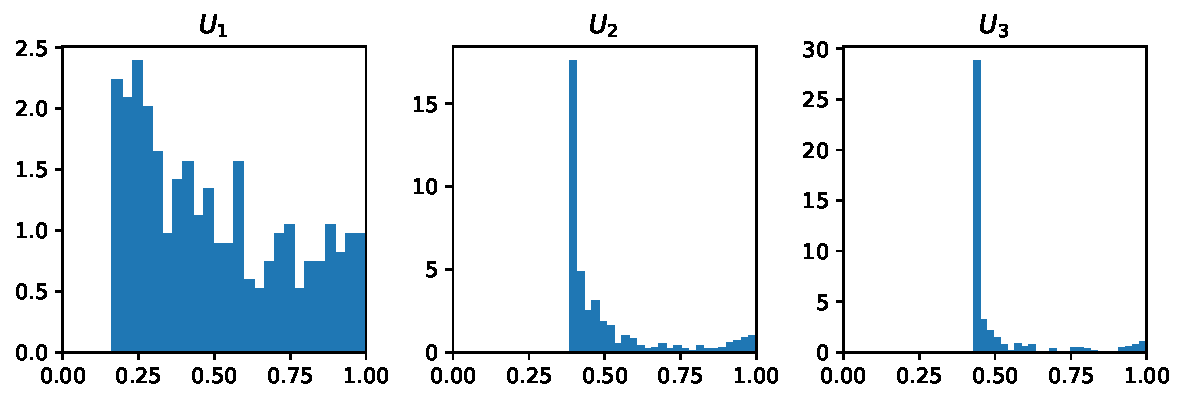
\includegraphics[width=0.99\linewidth]{figures/ND examples/Gaussian 3x3 large s uniforms.pdf}
        \caption{The samples transformed using $U_i = F_i(X_i)$ for $\boldsymbol\sigma = (1,2,3)$. These should be uniformly distributed, but clearly this is not the case for $U_2$ and $U_3$. Even $U_1$ does not quite resemble $10{,}000$ samples from a uniform distribution.}
        \label{fig:Gaussian 3x3 large s uniforms}
    \end{figure}
    Before handling this, the non-uniformity of $U_1$ in \autoref{fig:Gaussian 3x3 large s uniforms} is likely also present in the case when $\boldsymbol\sigma = (1,1,1)$. Indeed, \autoref{fig:Gaussian 3x3 medium s uniforms} shows that this is indeed the case.
    \begin{figure}[H]
        \centering
        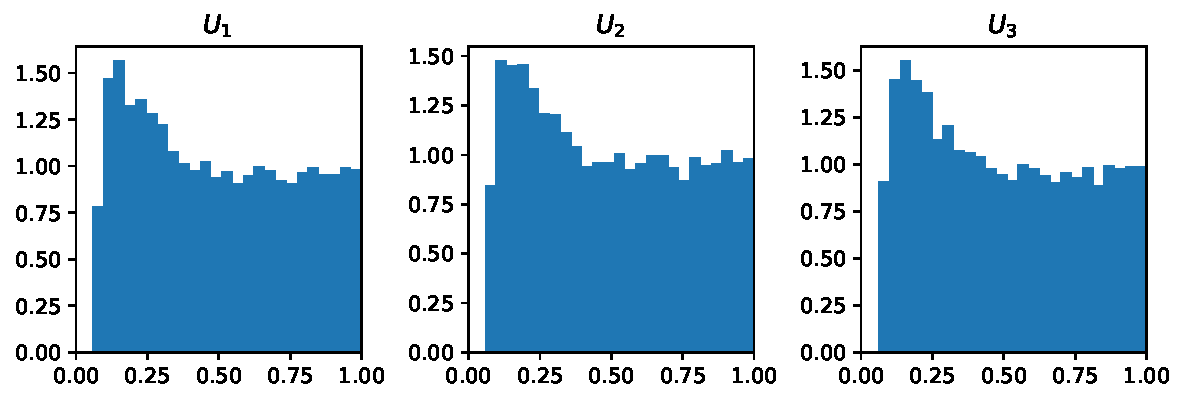
\includegraphics[width=0.99\linewidth]{figures/ND examples/Gaussian 3x3 medium s uniforms.pdf}
        \caption{The samples transformed using $U_i = F_i(X_i)$ for $\boldsymbol\sigma = (1,1,1)$.}
        \label{fig:Gaussian 3x3 medium s uniforms}
    \end{figure}
    Finally, just to be sure, $\boldsymbol\sigma = (0.07, 0.3, 0.9)$ is also shown in \autoref{fig:Gaussian 3x3 small s uniforms} and seems very reasonable, except for $U_3$.
    \begin{figure}[H]
        \centering
        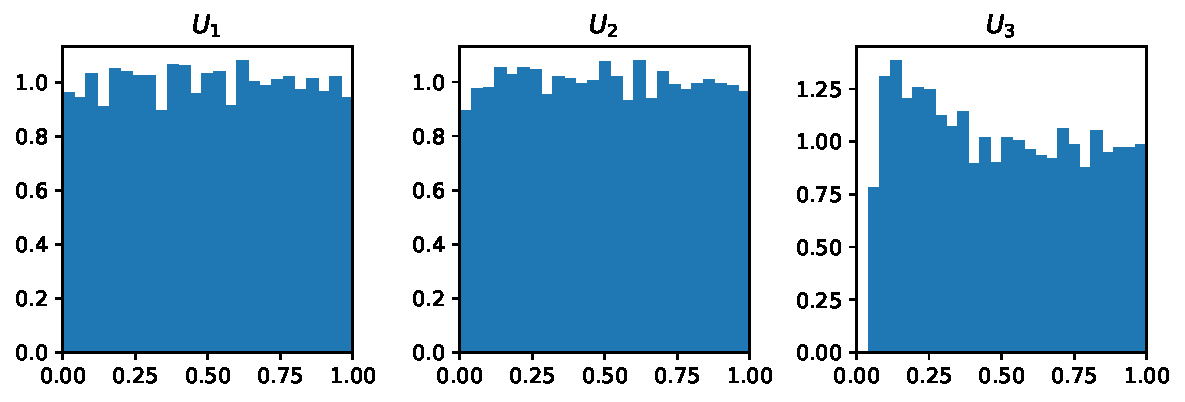
\includegraphics[width=0.99\linewidth]{figures/ND examples/Gaussian 3x3 small s uniforms.pdf}
        \caption{\raggedright The samples transformed using $U_i = F_i(X_i)$ for $\boldsymbol\sigma = (0.07, 0.3, 0.9)$.\hfill}
        \label{fig:Gaussian 3x3 small s uniforms}
    \end{figure}
    From the above examples, it seems that the larger the variance, the worse the uniforms turn out. Reasons for this could include numerical issues when trying to calculate $u_i^{(j)}$ form $y_i^{(j)}$ by $u_i^{(j)} = \int_{-\infty}^{y_i^{(j)}} f_i(y) \, dy$ and bad fitting of the kernel density estimate from observations. In particular, for values similar, which happens in the case for large $\sigma$ such that we observe large negative realizations of $X_i$, $y_i^{(j)}$ are almost 0, and when computing the integral could result in identical values. Furthermore, from \autoref{fig:Gaussian 3x3 large s X3 KDE} we see that indeed the fit is quite poor. Note that we have zoomed in on the interval $[-200 , 200]$ which contains $96.2\%$ of observations. The poor fit is primarily due to the use of Scott's Rule \textcolor{red}{as discussed above} which in this case overshoots the optimal bandwidth by a lot.
    \begin{figure}[H]
        \centering
        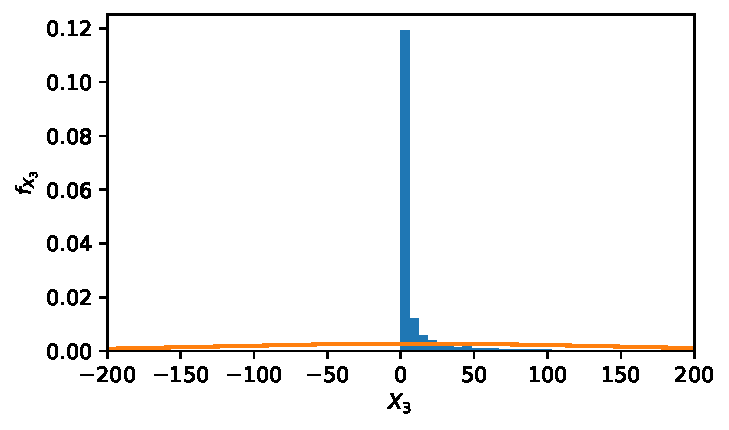
\includegraphics[width=0.7\linewidth]{figures/ND examples/Gaussian 3x3 large s X3 KDE.pdf}
        \caption{}
        \label{fig:Gaussian 3x3 large s X3 KDE}
    \end{figure}
    The poor fit also explains the high concentration of $U_3$ around $0.5$ in \autoref{fig:Gaussian 3x3 large s uniforms} as only $54.5\%$ of the probability mass lies above $0$.

    However, also here \autoref{coro: Coordinate transformation} proves to be useful. Namely, we can get rid of the numerical issues by transforming $Y_i$ using e.g. $\log(\cdot)$ or $(\cdot)^{p}$ for $p>0$ to get even out the observations more. As the first simply inverts the initial transformation of $X_i$, we choose the latter as a more interesting case. In particular, choosing $p<1$ will result in a more even distribution. In the following, $p=1/10$ has been used to transform $\boldsymbol Y$ prior to running \autoref{alg:Gobs1} and the resulting $u_i^{(j)}$ is shown in \autoref{fig:Gaussian 3x3 large s power uniforms}.
    \begin{figure}[H]
        \centering
        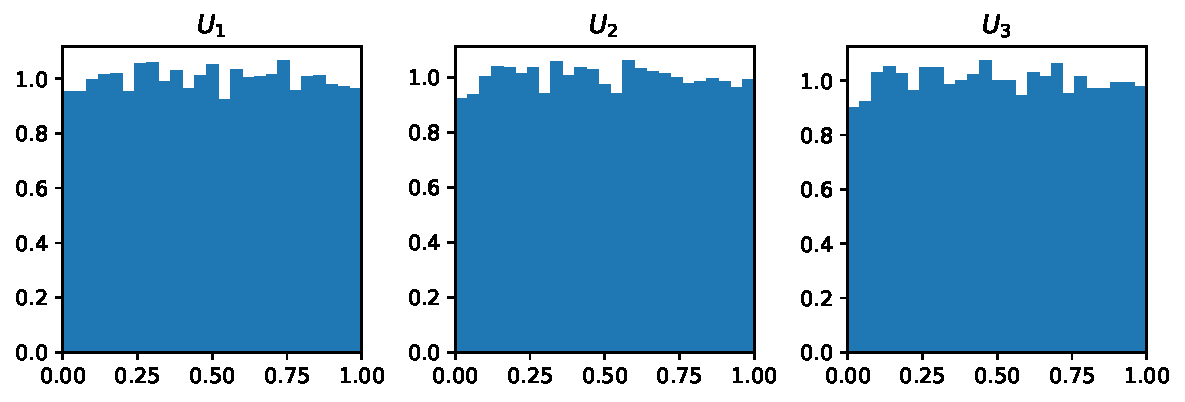
\includegraphics[width=0.99\linewidth]{figures/ND examples/Gaussian 3x3 large s power uniforms.pdf}
        \caption{}
        \label{fig:Gaussian 3x3 large s power uniforms}
    \end{figure}
    The resulting $u_i^{(j)}$ now seem to follow a uniform distribution and indeed the KDE fits much better as seen in \autoref{fig:Gaussian 3x3 large s power X3 KDE}.
    \begin{figure}[H]
        \centering
        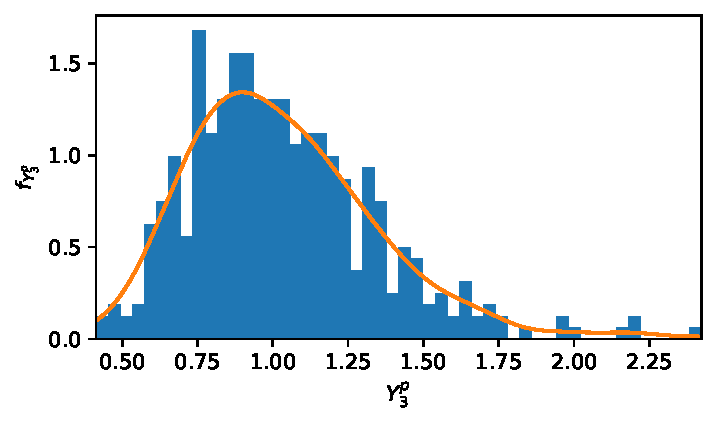
\includegraphics[width=0.7\linewidth]{figures/ND examples/Gaussian 3x3 large s power X3 KDE.pdf}
        \caption{}
        \label{fig:Gaussian 3x3 large s power X3 KDE}
    \end{figure}
    Turning to \autoref{alg:Gobs1} and \autoref{alg:ND} we now find that $G_{dir}$ is given by
    $$G_{dir} =
        \begin{bmatrix}
            -0.3290  & 0.6610   & 0.008440   \\
            0.6610   & -0.3290  & 0.008150   \\
            0.008440 & 0.008150 & -0.0002061
        \end{bmatrix}
    $$
    Which is indeed much more comparable with the result from before in \autoref{eq:s medium G_dir} and \autoref{eq:s small G_dir}. The difference between $G_{dir}$ from $\boldsymbol Y$ and $\boldsymbol Y^p$ is clearly visible in \autoref{fig:Gaussian 3x3 large s G_dir differences} and also \autoref{fig:Gaussian 3x3 large s power} resembles the original correlation structure.
    \begin{figure}[H]
        \centering
        \begin{subfigure}[t]{0.49\textwidth}
            \centering
            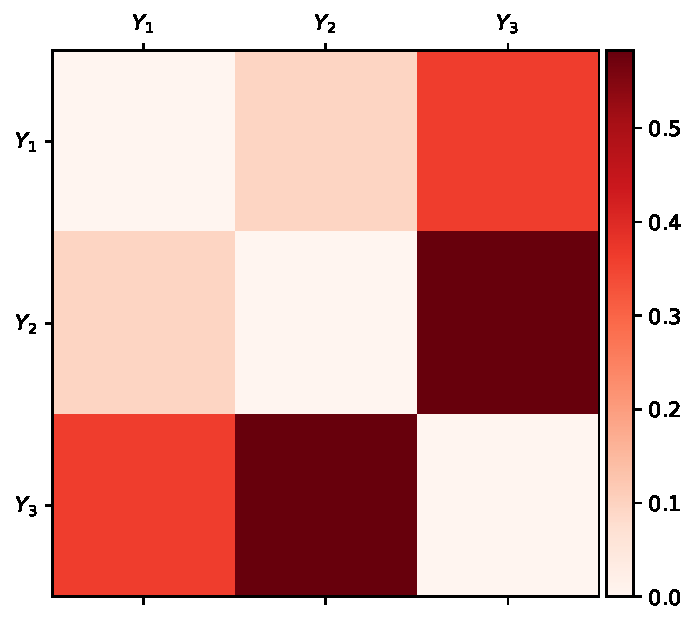
\includegraphics[width=\linewidth]{figures/ND examples/Gaussian 3x3 large s.pdf}
            \caption{}
            \label{fig:Gaussian 3x3 large s}
        \end{subfigure}%
        ~
        \begin{subfigure}[t]{0.49\textwidth}
            \centering
            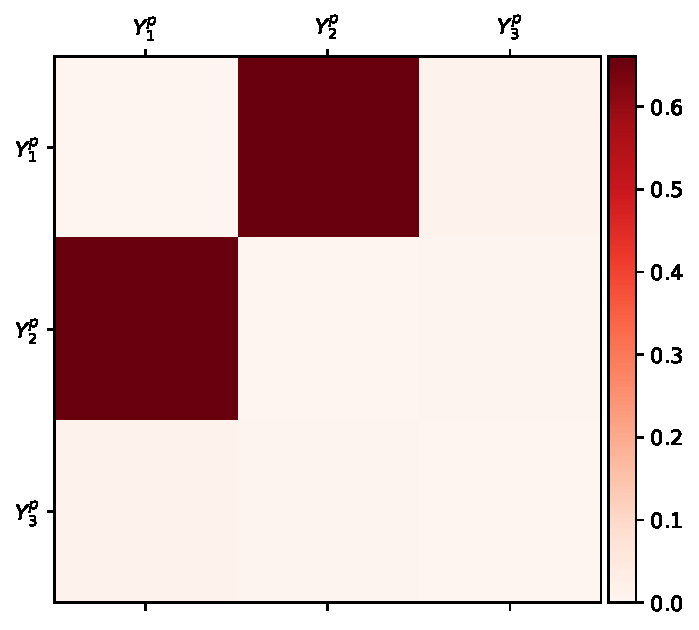
\includegraphics[width=\linewidth]{figures/ND examples/Gaussian 3x3 large s power.pdf}
            \caption{}
            \label{fig:Gaussian 3x3 large s power}
        \end{subfigure}
        \caption{$G_{dir}$ resulting from $10{,}000$ samples from multi variate Gaussian with $\boldsymbol\sigma = (1,2,3)$ in \textbf{(a)} with raw samples from $\boldsymbol Y$ and in \textbf{(b)} the transformed data corresponding to $\boldsymbol Y^p$.}
        \label{fig:Gaussian 3x3 large s G_dir differences}
    \end{figure}
    Finally, to end this example we shall compare with some theoretical results. Namely, the output $G_{obs}$ of \autoref{alg:Gobs1} can also be calculated theoretically. For this, we shall use \autoref{prop:MI bivariate gaussian} which permits a theoretical result, namely
    \begin{align*}
        G_{obs} & =
        \begin{bmatrix}
            0                                              & -\frac{1}{2} \ln \left( 1 - \rho_{12}^2\right) & -\frac{1}{2} \ln \left( 1 - \rho_{13}^2\right) \\
            -\frac{1}{2} \ln \left( 1 - \rho_{21}^2\right) & 0                                              & -\frac{1}{2} \ln \left( 1 - \rho_{23}^2\right) \\
            -\frac{1}{2} \ln \left( 1 - \rho_{31}^2\right) & -\frac{1}{2} \ln \left( 1 - \rho_{32}^2\right) & 0
        \end{bmatrix} \\
                & \cong
        \begin{bmatrix}
            0       & 0.83037 & 0 \\
            0.83037 & 0       & 0 \\
            0       & 0       & 0
        \end{bmatrix}
    \end{align*}
    Similarly, prior to deconvolution, using just the sampled $\boldsymbol X$ (i.e. no exponential transform), \autoref{alg:Gobs1} returns
    $$G_{obs} =
        \begin{bmatrix}
            0.         & 0.71841756 & 0.01781815 \\
            0.71841756 & 0.         & 0.01769672 \\
            0.01781815 & 0.01769672 & 0.
        \end{bmatrix}
    $$
    Clearly these are not equal, but in this case, the error is suspected to originate from the estimated joint density. For example, considering $X_1$ and $X_2$, we compare the estimated joint copula density and compare to the theoretical \textcolor{red}{reference til et sted hvor gausisk copula står} shown in \autoref{fig:gaussian copula estimate} and \autoref{fig:gaussian copula truth} respectively.
    \begin{figure}[H]
        \centering
        \begin{subfigure}[t]{0.45\linewidth}
            \centering
            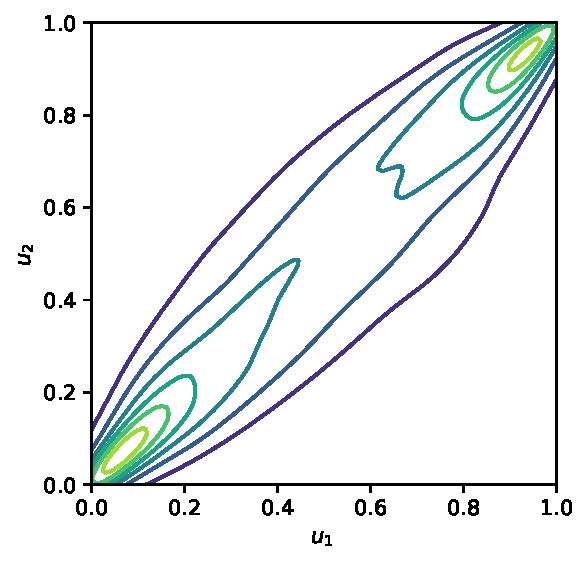
\includegraphics[width = \linewidth]{figures/ND examples/Gaussian copula sample contour.pdf}
            \caption{}
        \end{subfigure}%
        ~
        \begin{subfigure}[t]{0.5\linewidth}
            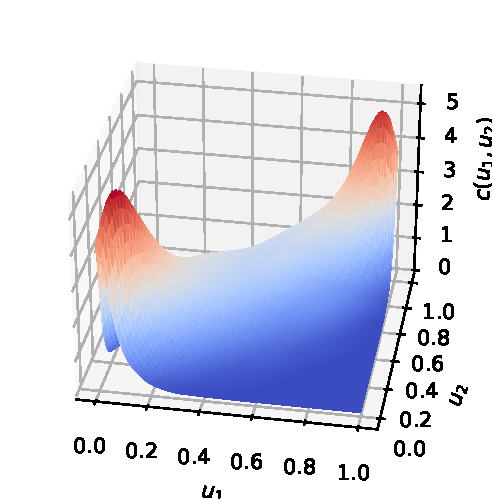
\includegraphics[width = \linewidth]{figures/ND examples/Gaussian copula sample pdf.pdf}
            \caption{}
        \end{subfigure}
        \caption{Estimated copula density $c$ with $\rho = 0.9$ corresponding to $X_1$ and $X_2$.}
        \label{fig:gaussian copula estimate}
    \end{figure}
    The noticeable difference is in the corners $(0,0)$ and $(1,1)$ where the theoretical copula density tends to infinity whereas the estimated density has modes at $(0.1,0.1)$ and $(0.9,0.9)$. In particular, simply rescaling the copula density in \autoref{alg:Gobs1} does not resemble the theoretical boundary which is a known issue \textcolor{red}{reference til artikel om undershoot peaks og boundary conditions for KDE}. A better approach may be to use jackknifing \textcolor{red}{link til afsnit of jackknifing, som også indeholder reference til artikel hvor dette gøres}.
    \begin{figure}[H]
        \centering
        \begin{subfigure}[t]{0.45\linewidth}
            \centering
            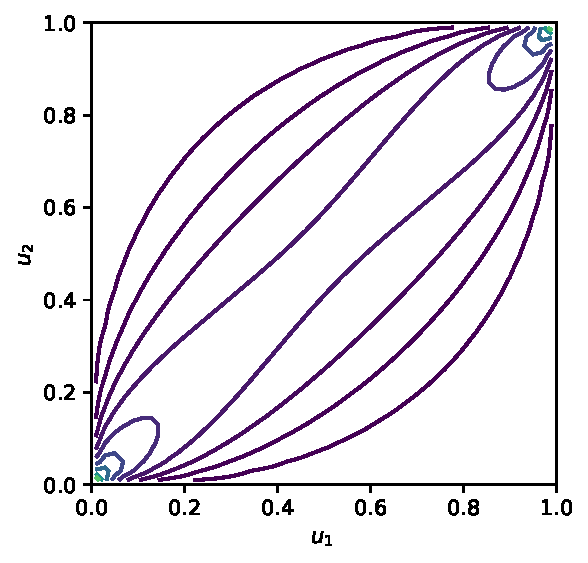
\includegraphics[width = \linewidth]{figures/ND examples/Gaussian copula theoretical contour.pdf}
            \caption{}
        \end{subfigure}%
        ~
        \begin{subfigure}[t]{0.5\linewidth}
            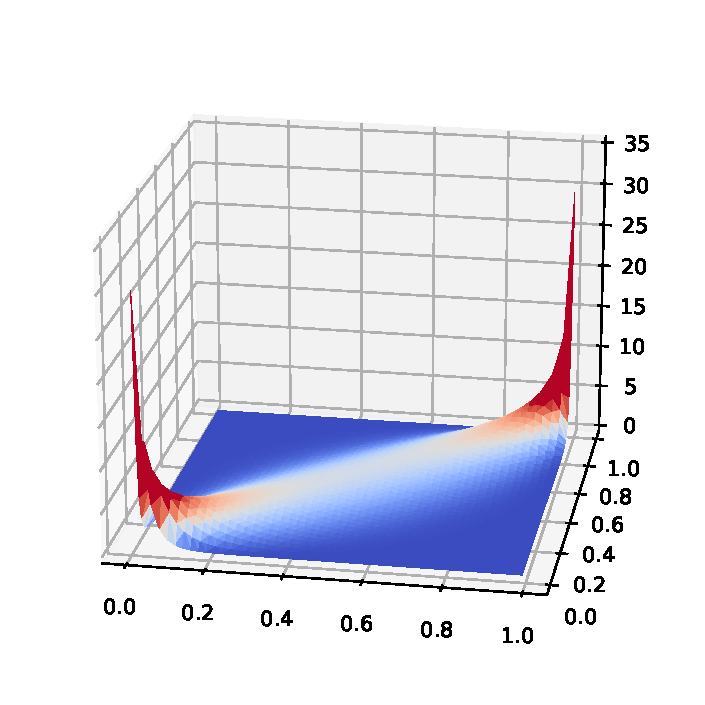
\includegraphics[width = \linewidth]{figures/ND examples/Gaussian copula theoretical pdf.pdf}
            \caption{}
        \end{subfigure}
        \caption{Theoretical copula density $c$ with $\rho = 0.9$ corresponding to $X_1$ and $X_2$.}
        \label{fig:gaussian copula truth}
    \end{figure}
    We note however, that the underlying structure is still captured i.e. that $Y_1$ and $Y_2$ covary while $Y_3$ does not inform $Y_1$ or $Y_2$ and vice versa.
\end{example}

We continue with a similar example to the previous one. The key difference is the number of variables and a more complicated correlation structure to test the algorithms further.
\begin{example}
    From \autoref{ex:1} we saw how one could handle some numerical issues. Thus, in this example we shall not bother ourselves with such computations and merely focus on the correlation structure. In particular, we shall sample $\boldsymbol X$ from a 10 dimensional
\end{example}


\newpage

\section{sammenligning af metoder for at finde MI}
Sammenligning af gammel metode og "min"
\begin{figure}[h]
    \centering
    \begin{subfigure}[t]{0.49\textwidth}
        \centering
        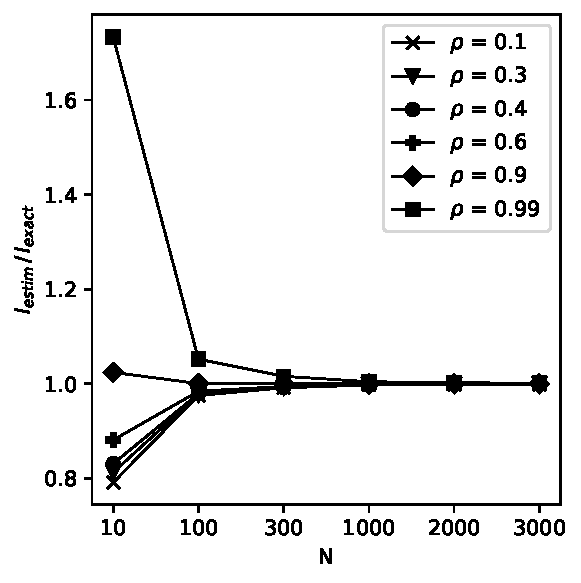
\includegraphics[width=\linewidth]{figures/ND examples/MI calc/gaussian example all.pdf}
        \caption{}
        \label{subfig:d}
    \end{subfigure}%
    ~
    \begin{subfigure}[t]{0.49\textwidth}
        \centering
        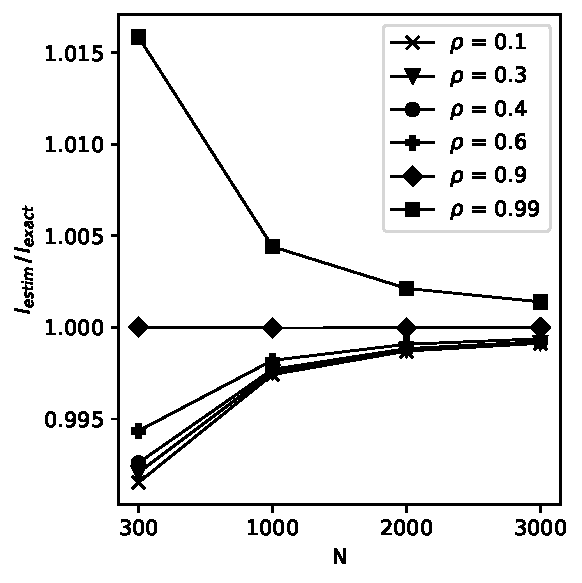
\includegraphics[width=\linewidth]{figures/ND examples/MI calc/gaussian example zoom.pdf}
        \caption{}
        \label{subfig:dd}
    \end{subfigure}
    \caption{Evaluation of MI for new method for different N. \textcolor{red}{Bør sammenlignes med artiekl fundet (har sat i bibtex) og original papers (ikke Kina)}}
    \label{fig:dd}
\end{figure}

\begin{figure}[h]
    \centering
    \begin{subfigure}[t]{0.32\textwidth}
        \centering
        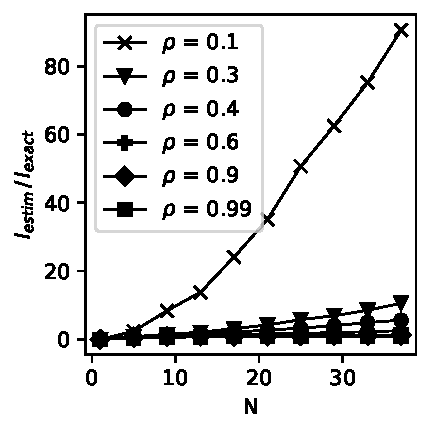
\includegraphics[width=\linewidth]{figures/ND examples/MI calc/gaussian example original all.pdf}
        \caption{}
        \label{subfig:d}
    \end{subfigure}%
    ~
    \begin{subfigure}[t]{0.32\textwidth}
        \centering
        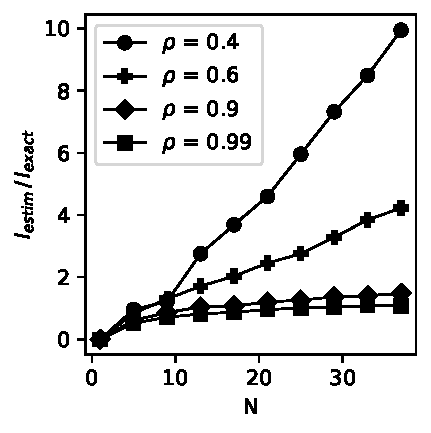
\includegraphics[width=\linewidth]{figures/ND examples/MI calc/gaussian example original zoom.pdf}
        \caption{}
        \label{subfig:dd}
    \end{subfigure}%
    ~
    \begin{subfigure}[t]{0.32\textwidth}
        \centering
        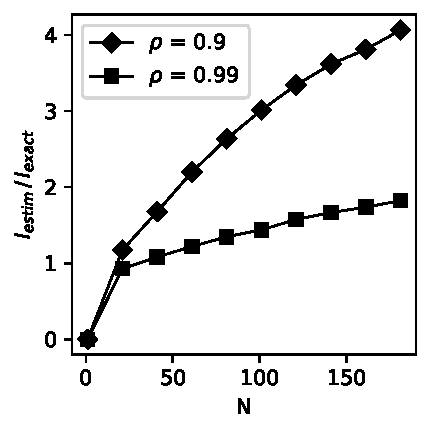
\includegraphics[width=\linewidth]{figures/ND examples/MI calc/gaussian example original high corr.pdf}
        \caption{}
        \label{subfig:dd}
    \end{subfigure}
    \caption{Evaluation of MI for old method for different N. Ligner der er knæk ved fporhold lig 1. Men ved næremere undersøgelse blev det fundet ud af at det ikke helt er tilfældet, og derudover vil der skulle laves en algoritmisk måde at finde dette knæk på. Savitzky–Golay filter kunne være en mulighed, eller gruppere e.g. 5 forskellige bins og tag gennemsnit. Efter smoothing kan anden afledte tæt på 0 bruges, til at finde hvornår stykket bliver fladt (tilnærmelses vist)}
    \label{fig:ddd}
\end{figure}


\textcolor{red}{Inkluder flere exempler end blot gaussian as done by \cite{Estimating-mutual-information-Kraskov}}

\end{document}










